\begin{figure}[t]
    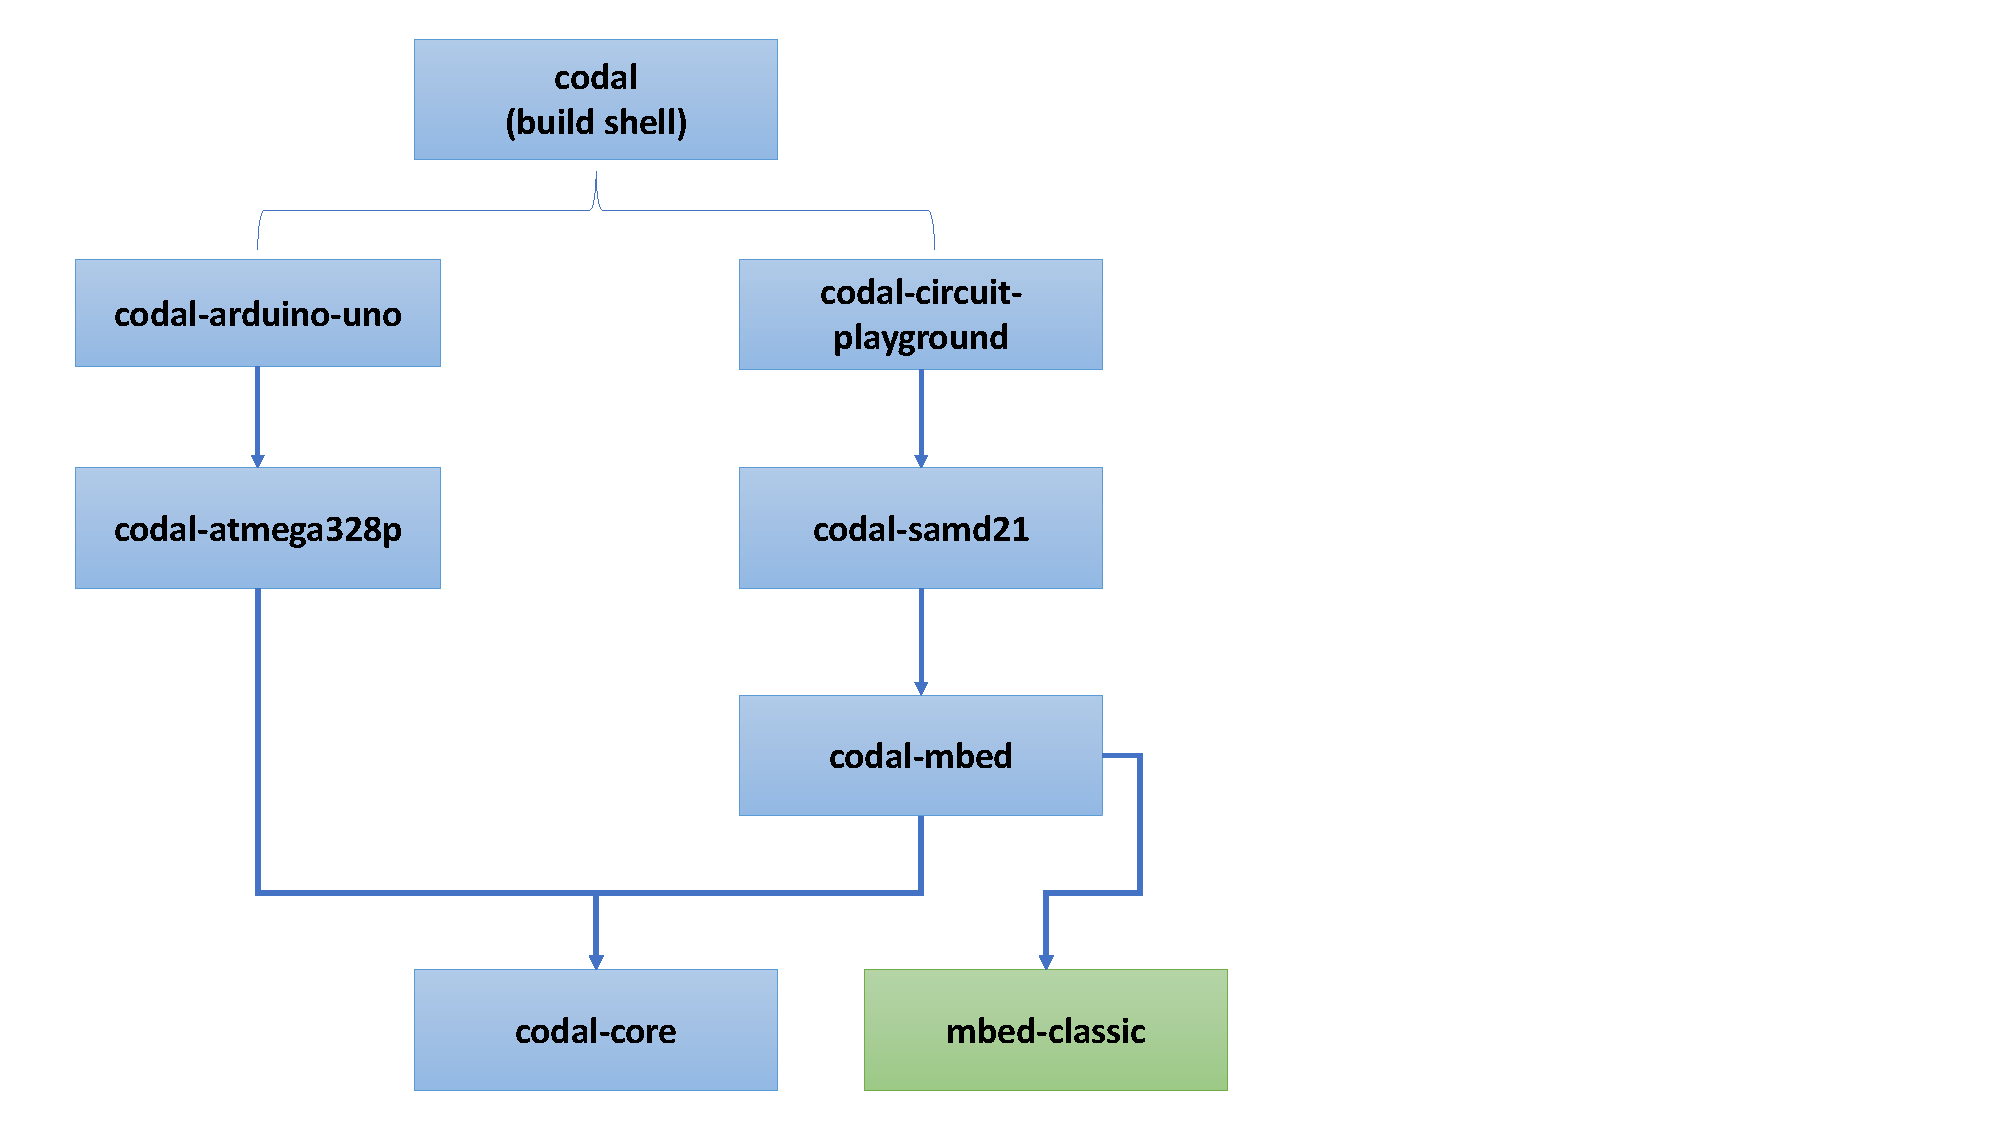
\includegraphics[width=4.5in]{codalFig.pdf}
    \caption{\label{fig:codal}Detailed relationships between \CO repos.}
\end{figure}

\section{The \CO Runtime}
\label{sec:codal}

The component-oriented device abstraction layer (\CO) is a multi-platform runtime designed to make efficient use of memory and energy, provide both synchronous and asynchronous API variants, and form a reasonable target for higher level languages
such as JavaScript.

\CO provides a set of components that abstract away microcontroller specifics, a non-preemptive scheduler that minimises the need for resource locking primitives whilst allowing asynchronous operation, and an eventing subsystem (common to all components) that enables the decoupling of system and user code. \CO components represent software or hardware drivers (an I2C device, a GPIO pin, a Message Bus, a Bluetooth device); any component can generate or consume events. \CO supports both polling and asynchronous (event-driven) programming models, which enables higher level languages to map straight onto native C/C++ APIs. Section~\ref{sec:related} compares \CO to other runtimes and operating systems for microcontrollers.

% more required here, needs to be reflowed...

\subsection{Structural Overview}

Figure~\ref{fig:codal} shows the repository architecture for two \CO devices, the Adafruit CircuitPlayground, built on top of ARM's mbed, and the Arduino Uno, built without any supporting libraries. The \COLN-core repo sits at the base of both device trees and provides the high level driver models which are implemented in the layer above. Each target library (\COLN-arduino-uno, \COLN-circuit-playground) builds on top of a processor library containing processor specific files, and the target library at the top of the tree contains files specific to a device --- commonly the linker script and the model for a device. A model is a C++ class that brings together components defined further down the tree as a single software representation of the device:

\begin{lstlisting}
class ArduinoUno : public CodalDevice
{
    ...

    public:

    ATMegaTimer                 timer;
    ATMegaSerial                serial;
    ArduinoIO                   io;
    ATMegaI2C                   i2c;
    MessageBus                  messageBus;

    ArduinoUno();
};
\end{lstlisting}

This architecture enables platform independent code to run across multiple processors and devices, while
allow for extensibility and specialisation.

\subsection{Message Bus and Events}

Message passing via events is a common technique and is the foundation of many operating systems --- yet in most systems events are static, used only to notify users of key events within the system (e.g. SIGKILL on UNIX).

In \CON, we offer extensible events where the data contained in an event can be arbitrary, and commonly application specific. Application developers can then ``listen'' to events, specifying an id (namespace), a value (unique within a namespace), and a function to be invoked when an event is raised. All events pass through the message bus, if a corresponding listener is in place, the function indicated by the listener is invoked. The eventing model aligns well to JavaScript and languages with event-based programming models. 

Not only do events enable easy modularisation of code, but they also safeguard the application programmer from situations where incorrect code could cause unexpected behaviour. Take for example an application to detect a button press, there are usually two solutions: (1) poll the state of a pin; or (2) configure an interrupt to fire when the state of a pin changes. Taking the latter approach, it could look something like this:

\begin{lstlisting}
int state = 0;

void buttonClicked() {
    int gpioState = PIN0;
    // button released, blink LED!
    if(state == 1 && gpioState == 0) {
        set_state(LED, 1);
        wait_ms(1000);
        set_state(LED, 0);
    }
    state = gpioState;
}

int main() {
    configure_interrupt(PIN0, buttonClicked);
    while(1);
}
\end{lstlisting}

The above code sample is considered bad practice as it prevents other interrupts (like Timers) from firing for at least a second when a button is released, however, this is often the first application that a user will create. Such frameworks advise users to avoid blocking functions and waiting in interrupt context, thus sidestepping the problem by punting responsibility to the user --- \CO uses the message bus abstraction to shield users from such scenarios:

\begin{lstlisting}
#include "CircuitPlayground.h"
CircuitPlayground cplay;

void buttonClicked() {
    cplay.io.led.setDigitalValue(1);
    cplay.sleep(1000);
    cplay.io.led.setDigitalValue(0);
}

int main() {
    cplay.messageBus.listen(ID_BUTTON_A,DEVICE_BUTTON_EVT_CLICK,buttonClicked);

    while(1) cplay.sleep(100);
}
\end{lstlisting}

Note that the user doesn't have to configure any interrupts, as they are handled by pre-existing drivers.

% Stuff to add (it's already quite long):
% * Provides a similar mechanism seen in higher level languages
% * Timer and queues?
% * message passing microkernel

\subsection{Fiber Scheduler}

Novice users often want to perform multiple operations concurrently, generally requiring threads. Threading is a confusing concept: users have to learn about locks, semaphores, and preemption, to prevent race conditions. Threads can also consume a large number of resources depending on the model that is adopted by the runtime environment.

\CO takes a non-preemptive scheduling approach which reduces the need for resource locking primitives. In \CON's scheduling model, fibers (a lightweight thread) are RAM efficient and have a variable stack size. As we adopt a non-preemptive scheduling model, user or driver code must call ``sleep'' to swap context to another thread, this means that at an invoke of sleep, the stack depth is small. When a fiber is paged out the entire stack is duplicated to the heap. This would normally be ill-advised, but due to a usually small stack size, this is more efficient than approaches where there is a mandated stack size.

Events and the message bus are integral to \CO even extending to fibers, which can block and wait on events to complete.

\subsection{Drivers}

Drivers are commonly low level interfaces that control external or integrated hardware on a device. For embedded developers, creating and using drivers involves translating datasheets into program code and using low-level interfaces, which can confuse novice programmers.

In \CON, drivers abstract away the complexities of the underlying hardware into reusable, extensible, easy-to-use components; for every hardware component there is a software component. There are three types of drivers in \CON: (1) an abstract specification of a driver model common to most devices (e.g. I2C, Serial); (2) a driver that relies only on the interfaces specified in a driver model  (e.g. an I2C based driver); and (3) the concrete implementation of the abstract driver model, which may be platform specific or platform agnostic. Not all devices are the same, and by generalising the interface, devices can introduce platform specific optimisations and specialisations.

Interrupts are integral to drivers: in Serial communications it is useful to know when a byte has been sent or received. As illustrated in the button example, performing operations in interrupt context can be detrimental to the device. \CO drivers use events to decouple computational tasks, that may take a variable length of time, from interrupt context.

% * motivation
% * example - I2C, microphone (DMA)
% * one component per piece of hardware or software
% * Provides a common interface
% * uses events to decouple from interrupt context.

\subsection{Memory Management}

Standard libraries in C++ do not offer reentrant versions of memory allocation calls like ``malloc'' and ``new'', forbidding the allocation of memory in interrupt context.

\CO implements its own heap allocater that is designed to safeguard users from the scenario above, introducing reentrant versions of malloc. The heap allocater is flexible, reconfigurable, and repurposable, allowing the specification of multiple heaps across memory and it is optimised for common sizes and repeat allocations.

\CO has a number of managed types that use reference counting to determine when memory should be freed. Internally, managed types use malloc to copy stack allocated data to the heap creating a safer environment for the user --- the reentrant behaviour of malloc and free are key here, as references can be created and destroyed regardless of processor context.
% * provides an interrupt safe environment for memory allocation
% * flexible implementation
%     - multiple heaps
%     - reconfigurable, repurposeable
% * optimisations for common sizes and repeated patterns
% * edu
% * couple of sentences on types
%     - ref counted, malloced types.

\subsection{Streams}
There are very few scenarios where a processor alone is used to accomplish a task, hence the growth in packaged devices where sensors are distributed alongside a main processing unit. With sensors on boarded, scenarios are centered on the processing, handling, and piping of information generated by sensors.

One scenario is the generation of audio data for a speaker, which has a specific clock rate at which buffers are consumed. Rate pacing the passing of audio buffers to the speaker is challenging --- should it be the users' responsibility to ensure buffers are delivered at the correct time?

In \CO, a Stream interface removes the complexity of these scenarios from user applications. Streams are formed of one source node (where data is generated), one sink node (where data is consumed), and 0 or more intermediate data streams which have knowledge of both upstream and downstream interfaces, forming a chain of filters and/or data processing units. Source nodes can push data into the stream, a sink node can pull data down the stream, and a data stream can do either (a Pull/Push model). This means that autonomous tasks can happen in the background, only requiring user intervention if the user application demands it.
The following code snippet will play a SawtoothTone whilst the device is powered on:
\begin{lstlisting}
CircuitPlayground cplay;
SAMD21DMAC dmac;
Synthesizer synth;
SAMD21DAC dac(cplay.io.speaker, dmac, synth.output, 44100);

int main()
{
    // Align sample rate to speaker DAC.
    synth.setSampleRate(dac.getSampleRate());
    synth.setTone(Synthesizer::SawtoothTone);
    synth.setFrequency(300);

    while(1) cplay.sleep(100);
}
\end{lstlisting}